% Options for packages loaded elsewhere
\PassOptionsToPackage{unicode}{hyperref}
\PassOptionsToPackage{hyphens}{url}
%
\documentclass[
  11pt,
  ignorenonframetext,
]{beamer}
\usepackage{pgfpages}
\setbeamertemplate{caption}[numbered]
\setbeamertemplate{caption label separator}{: }
\setbeamercolor{caption name}{fg=normal text.fg}
\beamertemplatenavigationsymbolsempty
% Prevent slide breaks in the middle of a paragraph
\widowpenalties 1 10000
\raggedbottom
\setbeamertemplate{part page}{
  \centering
  \begin{beamercolorbox}[sep=16pt,center]{part title}
    \usebeamerfont{part title}\insertpart\par
  \end{beamercolorbox}
}
\setbeamertemplate{section page}{
  \centering
  \begin{beamercolorbox}[sep=12pt,center]{part title}
    \usebeamerfont{section title}\insertsection\par
  \end{beamercolorbox}
}
\setbeamertemplate{subsection page}{
  \centering
  \begin{beamercolorbox}[sep=8pt,center]{part title}
    \usebeamerfont{subsection title}\insertsubsection\par
  \end{beamercolorbox}
}
\AtBeginPart{
  \frame{\partpage}
}
\AtBeginSection{
  \ifbibliography
  \else
    \frame{\sectionpage}
  \fi
}
\AtBeginSubsection{
  \frame{\subsectionpage}
}
\usepackage{amsmath,amssymb}
\usepackage{iftex}
\ifPDFTeX
  \usepackage[T1]{fontenc}
  \usepackage[utf8]{inputenc}
  \usepackage{textcomp} % provide euro and other symbols
\else % if luatex or xetex
  \usepackage{unicode-math} % this also loads fontspec
  \defaultfontfeatures{Scale=MatchLowercase}
  \defaultfontfeatures[\rmfamily]{Ligatures=TeX,Scale=1}
\fi
\usepackage{lmodern}
\usetheme[]{metropolis}
\ifPDFTeX\else
  % xetex/luatex font selection
\fi
% Use upquote if available, for straight quotes in verbatim environments
\IfFileExists{upquote.sty}{\usepackage{upquote}}{}
\IfFileExists{microtype.sty}{% use microtype if available
  \usepackage[]{microtype}
  \UseMicrotypeSet[protrusion]{basicmath} % disable protrusion for tt fonts
}{}
\makeatletter
\@ifundefined{KOMAClassName}{% if non-KOMA class
  \IfFileExists{parskip.sty}{%
    \usepackage{parskip}
  }{% else
    \setlength{\parindent}{0pt}
    \setlength{\parskip}{6pt plus 2pt minus 1pt}}
}{% if KOMA class
  \KOMAoptions{parskip=half}}
\makeatother
\usepackage{xcolor}
\newif\ifbibliography
\usepackage{color}
\usepackage{fancyvrb}
\newcommand{\VerbBar}{|}
\newcommand{\VERB}{\Verb[commandchars=\\\{\}]}
\DefineVerbatimEnvironment{Highlighting}{Verbatim}{commandchars=\\\{\}}
% Add ',fontsize=\small' for more characters per line
\newenvironment{Shaded}{}{}
\newcommand{\AlertTok}[1]{\textcolor[rgb]{1.00,0.00,0.00}{\textbf{#1}}}
\newcommand{\AnnotationTok}[1]{\textcolor[rgb]{0.38,0.63,0.69}{\textbf{\textit{#1}}}}
\newcommand{\AttributeTok}[1]{\textcolor[rgb]{0.49,0.56,0.16}{#1}}
\newcommand{\BaseNTok}[1]{\textcolor[rgb]{0.25,0.63,0.44}{#1}}
\newcommand{\BuiltInTok}[1]{\textcolor[rgb]{0.00,0.50,0.00}{#1}}
\newcommand{\CharTok}[1]{\textcolor[rgb]{0.25,0.44,0.63}{#1}}
\newcommand{\CommentTok}[1]{\textcolor[rgb]{0.38,0.63,0.69}{\textit{#1}}}
\newcommand{\CommentVarTok}[1]{\textcolor[rgb]{0.38,0.63,0.69}{\textbf{\textit{#1}}}}
\newcommand{\ConstantTok}[1]{\textcolor[rgb]{0.53,0.00,0.00}{#1}}
\newcommand{\ControlFlowTok}[1]{\textcolor[rgb]{0.00,0.44,0.13}{\textbf{#1}}}
\newcommand{\DataTypeTok}[1]{\textcolor[rgb]{0.56,0.13,0.00}{#1}}
\newcommand{\DecValTok}[1]{\textcolor[rgb]{0.25,0.63,0.44}{#1}}
\newcommand{\DocumentationTok}[1]{\textcolor[rgb]{0.73,0.13,0.13}{\textit{#1}}}
\newcommand{\ErrorTok}[1]{\textcolor[rgb]{1.00,0.00,0.00}{\textbf{#1}}}
\newcommand{\ExtensionTok}[1]{#1}
\newcommand{\FloatTok}[1]{\textcolor[rgb]{0.25,0.63,0.44}{#1}}
\newcommand{\FunctionTok}[1]{\textcolor[rgb]{0.02,0.16,0.49}{#1}}
\newcommand{\ImportTok}[1]{\textcolor[rgb]{0.00,0.50,0.00}{\textbf{#1}}}
\newcommand{\InformationTok}[1]{\textcolor[rgb]{0.38,0.63,0.69}{\textbf{\textit{#1}}}}
\newcommand{\KeywordTok}[1]{\textcolor[rgb]{0.00,0.44,0.13}{\textbf{#1}}}
\newcommand{\NormalTok}[1]{#1}
\newcommand{\OperatorTok}[1]{\textcolor[rgb]{0.40,0.40,0.40}{#1}}
\newcommand{\OtherTok}[1]{\textcolor[rgb]{0.00,0.44,0.13}{#1}}
\newcommand{\PreprocessorTok}[1]{\textcolor[rgb]{0.74,0.48,0.00}{#1}}
\newcommand{\RegionMarkerTok}[1]{#1}
\newcommand{\SpecialCharTok}[1]{\textcolor[rgb]{0.25,0.44,0.63}{#1}}
\newcommand{\SpecialStringTok}[1]{\textcolor[rgb]{0.73,0.40,0.53}{#1}}
\newcommand{\StringTok}[1]{\textcolor[rgb]{0.25,0.44,0.63}{#1}}
\newcommand{\VariableTok}[1]{\textcolor[rgb]{0.10,0.09,0.49}{#1}}
\newcommand{\VerbatimStringTok}[1]{\textcolor[rgb]{0.25,0.44,0.63}{#1}}
\newcommand{\WarningTok}[1]{\textcolor[rgb]{0.38,0.63,0.69}{\textbf{\textit{#1}}}}
\usepackage{longtable,booktabs,array}
\usepackage{calc} % for calculating minipage widths
\usepackage{caption}
% Make caption package work with longtable
\makeatletter
\def\fnum@table{\tablename~\thetable}
\makeatother
\usepackage{graphicx}
\makeatletter
\def\maxwidth{\ifdim\Gin@nat@width>\linewidth\linewidth\else\Gin@nat@width\fi}
\def\maxheight{\ifdim\Gin@nat@height>\textheight\textheight\else\Gin@nat@height\fi}
\makeatother
% Scale images if necessary, so that they will not overflow the page
% margins by default, and it is still possible to overwrite the defaults
% using explicit options in \includegraphics[width, height, ...]{}
\setkeys{Gin}{width=\maxwidth,height=\maxheight,keepaspectratio}
% Set default figure placement to htbp
\makeatletter
\def\fps@figure{htbp}
\makeatother
\setlength{\emergencystretch}{3em} % prevent overfull lines
\providecommand{\tightlist}{%
  \setlength{\itemsep}{0pt}\setlength{\parskip}{0pt}}
\setcounter{secnumdepth}{-\maxdimen} % remove section numbering
\ifLuaTeX
  \usepackage{selnolig}  % disable illegal ligatures
\fi
\IfFileExists{bookmark.sty}{\usepackage{bookmark}}{\usepackage{hyperref}}
\IfFileExists{xurl.sty}{\usepackage{xurl}}{} % add URL line breaks if available
\urlstyle{same}
\hypersetup{
  pdftitle={Análisis de presencias con procesos de puntos},
  pdfauthor={Gerardo Martín},
  hidelinks,
  pdfcreator={LaTeX via pandoc}}

\title{Análisis de presencias con procesos de puntos}
\subtitle{Tutorial intermedio de spatstat}
\author{Gerardo Martín}
\date{2022-06-29}

\begin{document}
\frame{\titlepage}

\hypertarget{simulaciuxf3n-de-presencias}{%
\section{Simulación de presencias}\label{simulaciuxf3n-de-presencias}}

\begin{frame}{Especificación de un centroide}
\protect\hypertarget{especificaciuxf3n-de-un-centroide}{}
\begin{center}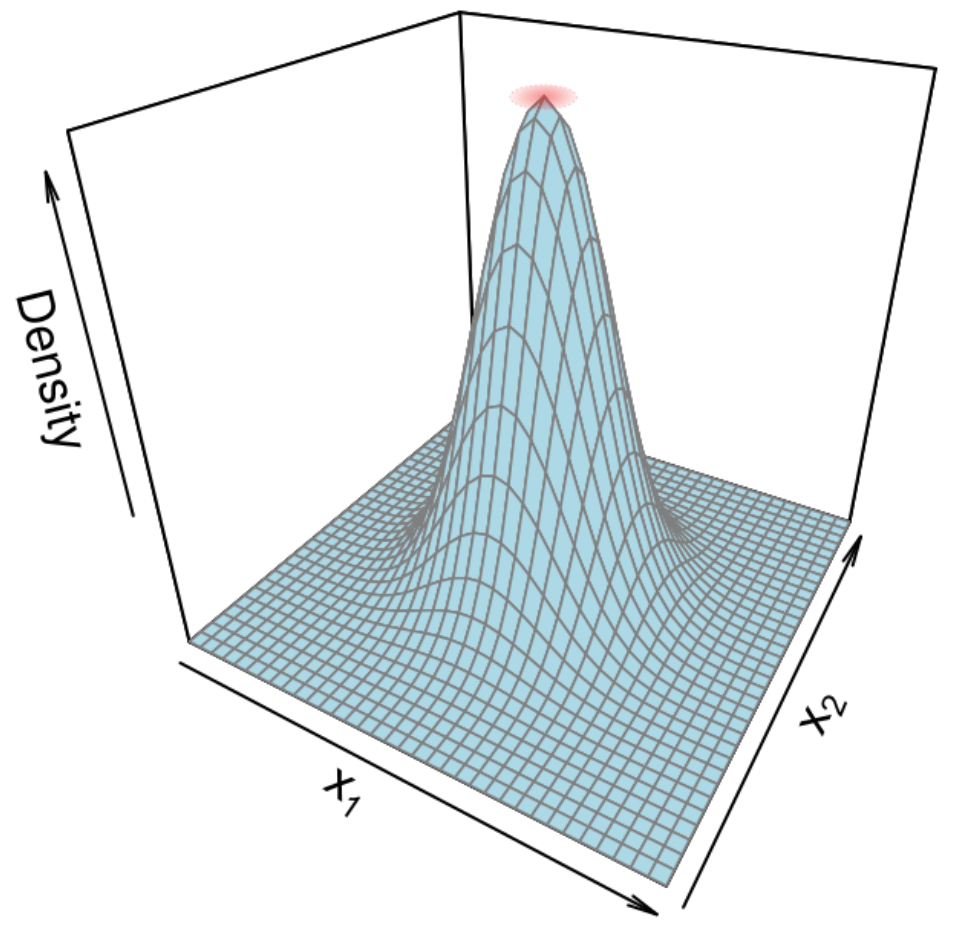
\includegraphics[width=13.28in]{Figuras/Centroide} \end{center}

\begin{itemize}
\tightlist
\item
  Abundancia alcanza un máximo y disminuye
\item
  Modelos más complicados con varias variables
\end{itemize}
\end{frame}

\hypertarget{anuxe1lisis-2}{%
\section{Análisis 2}\label{anuxe1lisis-2}}

\begin{frame}[fragile]{Importando y escalando datos y covariables}
\protect\hypertarget{importando-y-escalando-datos-y-covariables}{}
\begin{itemize}
\item
  \texttt{aggregate} disminuye la resolución por el factor indicado
\item
  \texttt{round} redondea los valores con el número de decimales
\item
  \textbf{Estos pasos no son enteramente necesarios en un análisis real,
  los hacemos para disminuir tiempo de cómputo}
\end{itemize}
\end{frame}

\begin{frame}{Código - viendo la favorabilidad}
\protect\hypertarget{cuxf3digo---viendo-la-favorabilidad}{}
\begin{center}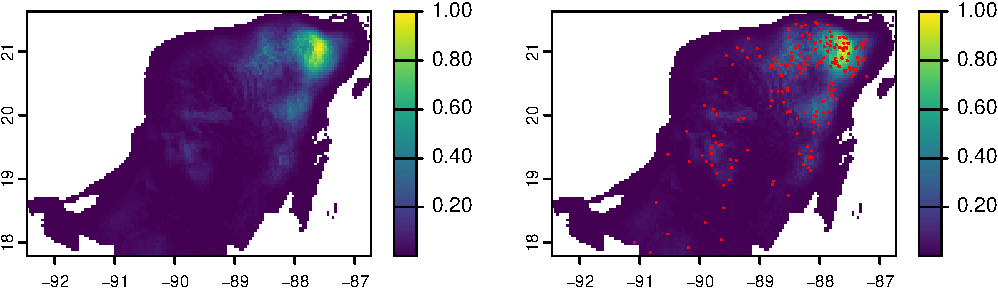
\includegraphics{Tutorial-spatstat-2_files/figure-beamer/unnamed-chunk-3-1} \end{center}
\end{frame}

\hypertarget{formateo-para-spatstat}{%
\section{Formateo para spatstat}\label{formateo-para-spatstat}}

\begin{frame}[fragile]{Cargando las funciones}
\protect\hypertarget{cargando-las-funciones}{}
\begin{Shaded}
\begin{Highlighting}[]
\FunctionTok{source}\NormalTok{(}\StringTok{"Funciones{-}spatstat/imFromStack.R"}\NormalTok{)}
\FunctionTok{source}\NormalTok{(}\StringTok{"Funciones{-}spatstat/plotQuantIntens.R"}\NormalTok{)}
\FunctionTok{source}\NormalTok{(}\StringTok{"Funciones{-}spatstat/findCompatibles.R"}\NormalTok{)}
\FunctionTok{source}\NormalTok{(}\StringTok{"Funciones{-}spatstat/getPolyFormulas.R"}\NormalTok{)}
\FunctionTok{source}\NormalTok{(}\StringTok{"Funciones{-}spatstat/ppmBatchFit.R"}\NormalTok{)}
\end{Highlighting}
\end{Shaded}
\end{frame}

\begin{frame}[fragile]{Formateo rápido}
\protect\hypertarget{formateo-ruxe1pido}{}
\begin{Shaded}
\begin{Highlighting}[]
\NormalTok{r.im }\OtherTok{\textless{}{-}} \FunctionTok{imFromStack}\NormalTok{(r)}
\FunctionTok{names}\NormalTok{(r.im) }\OtherTok{\textless{}{-}} \FunctionTok{names}\NormalTok{(r)}
\NormalTok{w }\OtherTok{\textless{}{-}} \FunctionTok{as.owin}\NormalTok{(r.im[[}\DecValTok{1}\NormalTok{]])}
\NormalTok{puntos.ppp }\OtherTok{\textless{}{-}} \FunctionTok{ppp}\NormalTok{(}\AttributeTok{x =}\NormalTok{ puntos}\SpecialCharTok{$}\NormalTok{x,}
                  \AttributeTok{y =}\NormalTok{ puntos}\SpecialCharTok{$}\NormalTok{y,}
                  \AttributeTok{window =}\NormalTok{ w,}
                  \AttributeTok{check =}\NormalTok{ F)}
\NormalTok{Q }\OtherTok{\textless{}{-}} \FunctionTok{pixelquad}\NormalTok{(}\AttributeTok{X =}\NormalTok{ puntos.ppp, }\AttributeTok{W =} \FunctionTok{as.owin}\NormalTok{(w))}
\end{Highlighting}
\end{Shaded}
\end{frame}

\hypertarget{anuxe1lisis-exploratorio}{%
\section{Análisis exploratorio}\label{anuxe1lisis-exploratorio}}

\begin{frame}{Autocorrelación}
\protect\hypertarget{autocorrelaciuxf3n}{}
Función de \emph{K} de Ripley

\begin{enumerate}
\tightlist
\item
  Número promedio de vecinos como función de la distancia a cada punto:
\end{enumerate}

\begin{figure}

{\centering 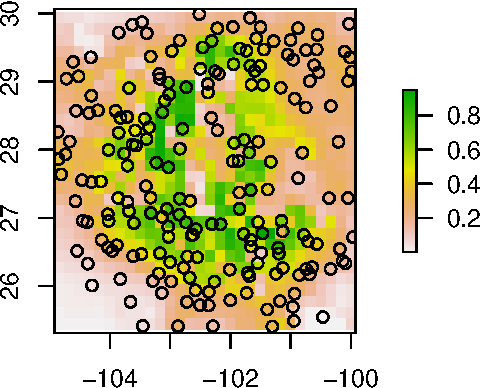
\includegraphics{Tutorial-spatstat-2_files/figure-beamer/unnamed-chunk-6-1} 

}

\caption{Buffers  de 0.1 a 0.5° alrededor de cada punto. El número de vecinos se cuenta por puntos dentro de cada buffer.}\label{fig:unnamed-chunk-6}
\end{figure}
\end{frame}

\begin{frame}{Los datos}
\protect\hypertarget{los-datos}{}
\begin{longtable}[]{@{}rr@{}}
\toprule\noalign{}
Radio & Vecinos \\
\midrule\noalign{}
\endhead
0.1 & 0.0000000 \\
0.2 & 0.0666667 \\
0.3 & 0.2000000 \\
0.4 & 0.2666667 \\
0.5 & 0.2666667 \\
\bottomrule\noalign{}
\end{longtable}
\end{frame}

\begin{frame}{Representación gráfica}
\protect\hypertarget{representaciuxf3n-gruxe1fica}{}
\begin{center}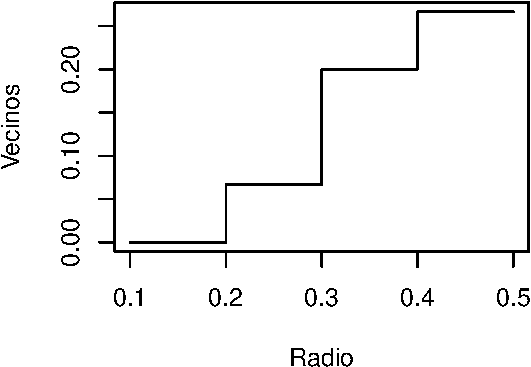
\includegraphics{Tutorial-spatstat-2_files/figure-beamer/unnamed-chunk-8-1} \end{center}
\end{frame}

\begin{frame}[fragile]{Implementación en spatstat}
\protect\hypertarget{implementaciuxf3n-en-spatstat}{}
\begin{Shaded}
\begin{Highlighting}[]
\NormalTok{K }\OtherTok{\textless{}{-}} \FunctionTok{envelope}\NormalTok{(puntos.ppp, }\AttributeTok{fun =}\NormalTok{ Kest, }\AttributeTok{nsim =} \DecValTok{39}\NormalTok{)}
\end{Highlighting}
\end{Shaded}

Para estimar significancia hace un muestreo aleatorios de punto, de ahí
que haya que especificar el número de simulaciones
(\texttt{nsim\ =\ 39}).
\end{frame}

\begin{frame}{Interpretación gráfica}
\protect\hypertarget{interpretaciuxf3n-gruxe1fica}{}
\begin{center}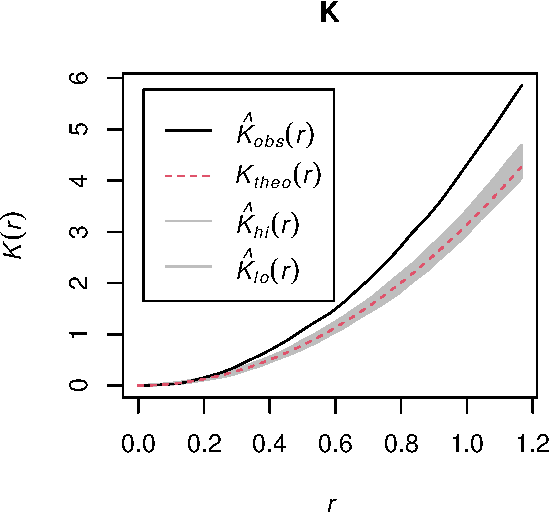
\includegraphics{Tutorial-spatstat-2_files/figure-beamer/unnamed-chunk-10-1} \end{center}
\end{frame}

\begin{frame}{Autocorrelación - notas}
\protect\hypertarget{autocorrelaciuxf3n---notas}{}
\begin{enumerate}
\item
  El proceso está levemente autocorrelacionado

  \begin{itemize}
  \tightlist
  \item
    Veremos si la correlación presente es explicada por factores
    ambientales
  \end{itemize}
\item
  No sabemos de momento si afectará al modelo
\end{enumerate}
\end{frame}

\hypertarget{anuxe1lisis-2.0}{%
\section{Análisis 2.0}\label{anuxe1lisis-2.0}}

\begin{frame}[fragile]{Respuestas a variables}
\protect\hypertarget{respuestas-a-variables}{}
\begin{Shaded}
\begin{Highlighting}[]
\FunctionTok{plotQuantIntens}\NormalTok{(}\AttributeTok{imList =}\NormalTok{ r.im,}
                \AttributeTok{noCuts =} \DecValTok{5}\NormalTok{,}
                \AttributeTok{Quad =}\NormalTok{ Q,}
                \AttributeTok{p.pp =}\NormalTok{ puntos.ppp,}
                \AttributeTok{dir =} \StringTok{""}\NormalTok{,}
                \AttributeTok{name =} \StringTok{"Respuestas{-}centroide"}\NormalTok{)}
\end{Highlighting}
\end{Shaded}

\href{Respuestas-centroide.pdf}{Ver archivo de gráficas}
\end{frame}

\begin{frame}[fragile]{Consideraciones para proponer modelos}
\protect\hypertarget{consideraciones-para-proponer-modelos}{}
Curvas con forma de campana \(\rightarrow\) fórmula cuadrática

\begin{Shaded}
\begin{Highlighting}[]
\FunctionTok{curve}\NormalTok{(}\FunctionTok{exp}\NormalTok{(}\DecValTok{1} \SpecialCharTok{+}\NormalTok{ x }\SpecialCharTok{{-}}\NormalTok{ x}\SpecialCharTok{\^{}}\DecValTok{2}\NormalTok{), }\AttributeTok{from =} \SpecialCharTok{{-}}\DecValTok{3}\NormalTok{, }\DecValTok{3}\NormalTok{)}
\end{Highlighting}
\end{Shaded}

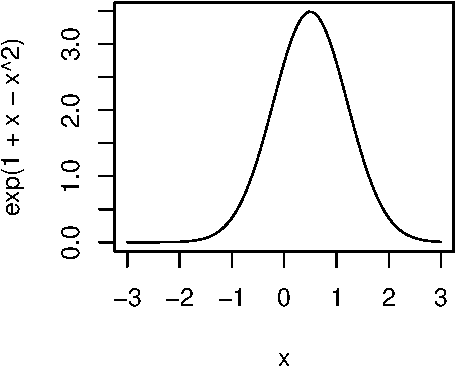
\includegraphics{Tutorial-spatstat-2_files/figure-beamer/unnamed-chunk-12-1.pdf}
\end{frame}

\begin{frame}{Consideraciones para proponer modelos}
\protect\hypertarget{consideraciones-para-proponer-modelos-1}{}
Ecuación lineal:

\[ y = \alpha + \beta_1 x_1 + \dots + \beta_n x_n\] Ecuación polinomial
de 2\(^o\) grado

\[ y = \alpha + \beta_1 x_1 + \beta_1' x_1^2 + \dots + \beta_n x_n + \beta_n' x_n^2\]
Recordemos que \(y = \log \lambda\)
\end{frame}

\begin{frame}[fragile]{¿Qué variables podemos incluir en el mismo
modelo?}
\protect\hypertarget{quuxe9-variables-podemos-incluir-en-el-mismo-modelo}{}
\textbf{Regla de oro}: Aquellas que no estén correlacionadas

\begin{itemize}
\tightlist
\item
  Que \(x_1\) no sea predictor de \(x_2\)
\item
  No se puede atribuir efecto de \(x_1\) ó \(x_2\) sobre \(\lambda\)
\item
  Necesitamos medir correlación entre pares de variables
  (\texttt{pairs})
\end{itemize}
\end{frame}

\begin{frame}[fragile]{Identificación automática de covariables
\emph{compatibles}}
\protect\hypertarget{identificaciuxf3n-automuxe1tica-de-covariables-compatibles}{}
\begin{Shaded}
\begin{Highlighting}[]
\NormalTok{compatibles }\OtherTok{\textless{}{-}} \FunctionTok{findCompatibles}\NormalTok{(r, }\AttributeTok{thres =} \FloatTok{0.5}\NormalTok{, }
                               \AttributeTok{max.comb =} \DecValTok{3}\NormalTok{)}
\end{Highlighting}
\end{Shaded}

\begin{longtable}[]{@{}lll@{}}
\toprule\noalign{}
Variable\_1 & Variable\_2 & Variable\_3 \\
\midrule\noalign{}
\endhead
bio1 & bio12 & bio18 \\
bio1 & bio12 & bio2 \\
bio1 & bio12 & bio3 \\
bio1 & bio12 & bio4 \\
bio1 & bio12 & bio6 \\
bio1 & bio12 & bio7 \\
\bottomrule\noalign{}
\end{longtable}
\end{frame}

\begin{frame}[fragile]{Obteniendo las fórmulas}
\protect\hypertarget{obteniendo-las-fuxf3rmulas}{}
\begin{itemize}
\item
  Necesitamos generar una tabla de exponentes para variables, usando el
  resultado de
  \href{Respuestas-centroide.pdf}{\texttt{plotQuantIntens}}.
\item
  Razonamiento:

  \begin{itemize}
  \item
    Identificar exponente máximo que tendrá el modelo para cada variable
  \item
    La función \texttt{getPolyFormulas} generará las fórmulas para todas
    las combinaciones con exponentes \(1:n\)
  \end{itemize}
\item
  Tabla debe tener dos columnas: \texttt{Variable}, \texttt{Power}
\end{itemize}
\end{frame}

\begin{frame}[fragile]{Uso de \texttt{getPolyFormulas}}
\protect\hypertarget{uso-de-getpolyformulas}{}
\begin{Shaded}
\begin{Highlighting}[]
\NormalTok{expon }\OtherTok{\textless{}{-}} \FunctionTok{read.csv}\NormalTok{(}\StringTok{"Datos/Tabla{-}coefs.csv"}\NormalTok{)}
\NormalTok{formulas  }\OtherTok{\textless{}{-}} \FunctionTok{getPolyFormulas}\NormalTok{(}\AttributeTok{respDF =}\NormalTok{ expon, }
                             \AttributeTok{compatMat =}\NormalTok{ compatibles)}
\NormalTok{formulas[}\DecValTok{1}\SpecialCharTok{:}\DecValTok{5}\NormalTok{]}
\end{Highlighting}
\end{Shaded}

\begin{verbatim}
## [1] "~bio1 + bio12 + I(bio12^2) + bio18 + I(bio18^2) + I(bio18^3) + I(bio18^4)"
## [2] "~bio1 + bio12 + I(bio12^2) + bio2 + I(bio2^2)"                            
## [3] "~bio1 + bio12 + I(bio12^2) + bio3 + I(bio3^2)"                            
## [4] "~bio1 + bio12 + I(bio12^2) + bio4 + I(bio4^2)"                            
## [5] "~bio1 + bio12 + I(bio12^2) + bio6 + I(bio6^2)"
\end{verbatim}
\end{frame}

\begin{frame}[fragile]{Ajustando los modelos}
\protect\hypertarget{ajustando-los-modelos}{}
\begin{itemize}
\item
  La función \texttt{ppmBatchFit} ajustará todos los modelos generados
  por \texttt{getPolyFormulas}
\item
  Algunos modelos no lograrán estimar coeficientes satisfactoriamente
\item
  La implementación presente solamente puede priorizar con base en AIC
\item
  En un futuro, eliminará modelos que con converjan
\end{itemize}
\end{frame}

\begin{frame}[fragile]{Uso de \texttt{ppmBatcchFit}}
\protect\hypertarget{uso-de-ppmbatcchfit}{}
\begin{Shaded}
\begin{Highlighting}[]
\NormalTok{modelos }\OtherTok{\textless{}{-}} \FunctionTok{ppmBatchFit}\NormalTok{(}\AttributeTok{points =}\NormalTok{ puntos,}
                       \AttributeTok{covariates =}\NormalTok{ r, }
                       \AttributeTok{formulas =}\NormalTok{ formulas[}\DecValTok{1}\SpecialCharTok{:}\DecValTok{10}\NormalTok{],}
                       \AttributeTok{parallel =}\NormalTok{ F,}
                       \AttributeTok{topModels =} \DecValTok{5}\NormalTok{)}
\end{Highlighting}
\end{Shaded}
\end{frame}

\begin{frame}[fragile]{Los argumentos}
\protect\hypertarget{los-argumentos}{}
\begin{itemize}
\item
  \texttt{points}, tabla de coordenadas con dos columnas, \texttt{x} y
  \texttt{y}, en formato \texttt{data.frame}
\item
  \texttt{covariates}, raster con bandas como covariables, nombres deben
  coincidir con fórmulas
\item
  \texttt{formulas}
\item
  \texttt{parallel}, si la rutina se ejeccutará en serie ó paralelo, si
  \texttt{parallel\ =\ T}, especificar número de núcleos a usar con
  \texttt{cores\ =\ 3} (ajustar para cada máquina)
\item
  \texttt{topModels}, cuántos de los ``mejores'' modelos queremos que
  nos guarde
\item
  El resultado almacenado en \texttt{modelos} es una lista con los 5
  mejores con base en el AIC
\end{itemize}
\end{frame}

\begin{frame}[fragile]{Analizando el resultado}
\protect\hypertarget{analizando-el-resultado}{}
\begin{Shaded}
\begin{Highlighting}[]
\FunctionTok{sapply}\NormalTok{(modelos, AIC)}
\end{Highlighting}
\end{Shaded}

\begin{verbatim}
## [1]  -936.8556  -953.2552  -945.1438 -1031.7370  -956.3632
\end{verbatim}

Podemos usar los procedimientos habituales para los modelos de regresión
en R

\begin{Shaded}
\begin{Highlighting}[]
\FunctionTok{summary}\NormalTok{(modelos[[}\DecValTok{1}\NormalTok{]])}
\end{Highlighting}
\end{Shaded}
\end{frame}

\begin{frame}[fragile]{Análisis de residuales}
\protect\hypertarget{anuxe1lisis-de-residuales}{}
Como en los análisis de regresión, podemos ver el ajuste con los
residuales, y siendo un modelo espacial, ver si hemos logrado explicar
la correlación espacial con la prueba \(K\) de Ripley, tal como en el
análisis exploratorio:

\begin{Shaded}
\begin{Highlighting}[]
\NormalTok{K.modelo }\OtherTok{\textless{}{-}} \FunctionTok{envelope}\NormalTok{(modelos[[}\DecValTok{1}\NormalTok{]], }\AttributeTok{fun =} \StringTok{"Kest"}\NormalTok{, }\AttributeTok{nsim =} \DecValTok{39}\NormalTok{)}
\end{Highlighting}
\end{Shaded}

\begin{verbatim}
## Generating 39 simulated realisations of fitted Poisson model  ...
## 1, 2, 3, 4, 5, 6, 7, 8, 9, 10, 11, 12, 13, 14, 15, 16, 17, 18, 19, 20,
## 21, 22, 23, 24, 25, 26, 27, 28, 29, 30, 31, 32, 33, 34, 35, 36, 37, 38, 
## 39.
## 
## Done.
\end{verbatim}

Esta prueba genera 39 patrones de puntos utilizando el modelo base para
calcular la función de Ripley y compara las simulaciones con la base de
datos
\end{frame}

\begin{frame}[fragile]{Gráfica}
\protect\hypertarget{gruxe1fica}{}
\begin{Shaded}
\begin{Highlighting}[]
\FunctionTok{par}\NormalTok{(}\AttributeTok{mfrow =} \FunctionTok{c}\NormalTok{(}\DecValTok{1}\NormalTok{, }\DecValTok{2}\NormalTok{))}
\FunctionTok{plot}\NormalTok{(K, }\AttributeTok{main =} \StringTok{"Datos"}\NormalTok{)}
\FunctionTok{plot}\NormalTok{(K.modelo, }\AttributeTok{main =} \StringTok{"Modelo"}\NormalTok{)}
\end{Highlighting}
\end{Shaded}

\begin{center}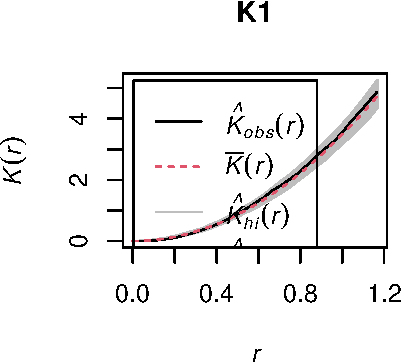
\includegraphics{Tutorial-spatstat-2_files/figure-beamer/unnamed-chunk-20-1} \end{center}
\end{frame}

\begin{frame}{Métodos para residuales}
\protect\hypertarget{muxe9todos-para-residuales}{}
\begin{itemize}
\item
  Gráficas de horizonte
\item
  Muestra 4 páneles:
\end{itemize}

\begin{enumerate}
\tightlist
\item
  Patrón de puntos
\item
  Residuales acumulados en cada fila de píxeles
\item
  Residuales acumulados en cada columna de píxeles
\item
  Residuales suavizados con contornos:
\end{enumerate}

\[Kernel - Modelo\]
\end{frame}

\begin{frame}[fragile]{Gráfica de horizonte}
\protect\hypertarget{gruxe1fica-de-horizonte}{}
\begin{Shaded}
\begin{Highlighting}[]
\FunctionTok{par}\NormalTok{(}\AttributeTok{mar =} \FunctionTok{c}\NormalTok{(}\FloatTok{1.5}\NormalTok{,}\DecValTok{1}\NormalTok{,}\DecValTok{0}\NormalTok{,}\DecValTok{0}\NormalTok{))}
\FunctionTok{diagnose.ppm}\NormalTok{(modelos[[}\DecValTok{1}\NormalTok{]], }\AttributeTok{cex =} \FloatTok{0.25}\NormalTok{, }\AttributeTok{outer =} \DecValTok{5}\NormalTok{)}
\end{Highlighting}
\end{Shaded}

\begin{center}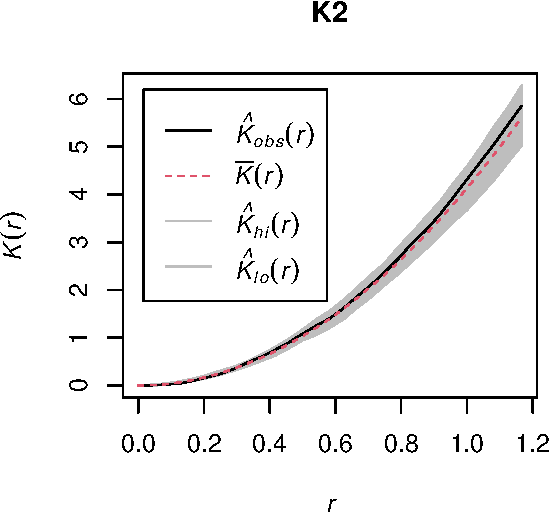
\includegraphics{Tutorial-spatstat-2_files/figure-beamer/unnamed-chunk-21-1} \end{center}

\begin{verbatim}
## Model diagnostics (raw residuals)
## Diagnostics available:
##  four-panel plot
##  mark plot 
##  smoothed residual field
##  x cumulative residuals
##  y cumulative residuals
##  sum of all residuals
## sum of raw residuals in entire window = -1.465e-06
## area of entire window = 11.3
## quadrature area = 11.28
## range of smoothed field =  [-13.75, 17.05]
\end{verbatim}
\end{frame}

\hypertarget{correcciuxf3n-de-sesgo}{%
\section{Corrección de sesgo}\label{correcciuxf3n-de-sesgo}}

\begin{frame}[fragile]{Definición de escenario de sesgo}
\protect\hypertarget{definiciuxf3n-de-escenario-de-sesgo}{}
\begin{Shaded}
\begin{Highlighting}[]
\NormalTok{sesgo }\OtherTok{\textless{}{-}} \FunctionTok{rast}\NormalTok{(}\FunctionTok{c}\NormalTok{(}\StringTok{"Datos/Target{-}group.tif"}\NormalTok{, }
                \StringTok{"Datos/Distance{-}roads.tif"}\NormalTok{))}
\NormalTok{sesgo }\OtherTok{\textless{}{-}} \FunctionTok{resample}\NormalTok{(sesgo, r)}
\FunctionTok{plot}\NormalTok{(sesgo)}
\end{Highlighting}
\end{Shaded}

\begin{center}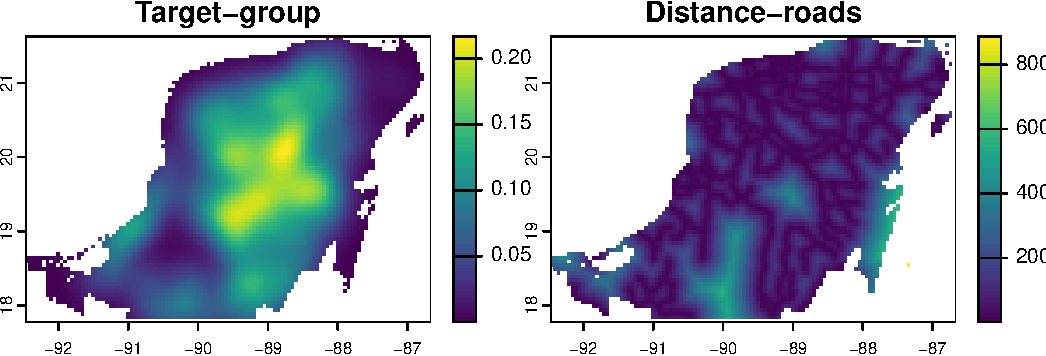
\includegraphics{Tutorial-spatstat-2_files/figure-beamer/unnamed-chunk-22-1} \end{center}
\end{frame}

\begin{frame}[fragile]{Filtrado del entorno}
\protect\hypertarget{filtrado-del-entorno}{}
\begin{itemize}
\tightlist
\item
  Usaremos las función \texttt{maskBias}
\end{itemize}

\begin{Shaded}
\begin{Highlighting}[]
\FunctionTok{source}\NormalTok{(}\StringTok{"Funciones{-}spatstat/maskBias.R"}\NormalTok{)}
\end{Highlighting}
\end{Shaded}

\begin{itemize}
\tightlist
\item
  Necesita los siguientes argumentos:
\end{itemize}

\begin{enumerate}
\tightlist
\item
  \texttt{s}, es el raster multi-banda de las covariables
\item
  \texttt{pres.areas}, es la base de datos de presencia con las
  coordenadas \texttt{x} y \texttt{y}
\item
  \texttt{bias.lay}, la capa que representa el esfuerzo de muestreo,
  donde los valores máximos correspondan a aquellos más muestreados.
\item
  \texttt{p.keep}, la proporción de valores a ser retenidos en cada
  corte de la capa
\item
  \texttt{power}, cuánto queremos que las muestras se concentren en los
  valores más altos de la capa de sesgo
\item
  \texttt{dis}, un factor de desagregación en caso que querer concentrar
  más valores en las zonas más muestreadas de lo que la resolución
  presente permite (muuy costoso actualmente)
\end{enumerate}
\end{frame}

\begin{frame}[fragile]{Ejemplos}
\protect\hypertarget{ejemplos}{}
\begin{Shaded}
\begin{Highlighting}[]
\NormalTok{r.mask1 }\OtherTok{\textless{}{-}} \FunctionTok{maskBias}\NormalTok{(}\AttributeTok{s =}\NormalTok{ r[[}\DecValTok{1}\NormalTok{]], }\CommentTok{\#Bio1}
                   \AttributeTok{pres.areas =}\NormalTok{ puntos, }
                   \AttributeTok{bias.lay =}\NormalTok{ sesgo[[}\DecValTok{1}\NormalTok{]], }\CommentTok{\#Target group}
                   \AttributeTok{p.keep =} \FloatTok{0.1}\NormalTok{, }\AttributeTok{power =} \DecValTok{1}\NormalTok{)}

\NormalTok{r.mask2 }\OtherTok{\textless{}{-}} \FunctionTok{maskBias}\NormalTok{(}\AttributeTok{s =}\NormalTok{ r[[}\DecValTok{1}\NormalTok{]], }\CommentTok{\#Bio1}
                   \AttributeTok{pres.areas =}\NormalTok{ puntos, }
                   \AttributeTok{bias.lay =}\NormalTok{ sesgo[[}\DecValTok{1}\NormalTok{]], }\CommentTok{\#Target group}
                   \AttributeTok{p.keep =} \FloatTok{0.1}\NormalTok{, }\AttributeTok{power =} \DecValTok{3}\NormalTok{, }\AttributeTok{dis =} \DecValTok{4}\NormalTok{)}
\end{Highlighting}
\end{Shaded}
\end{frame}

\begin{frame}{Gráfica}
\protect\hypertarget{gruxe1fica-1}{}
\begin{center}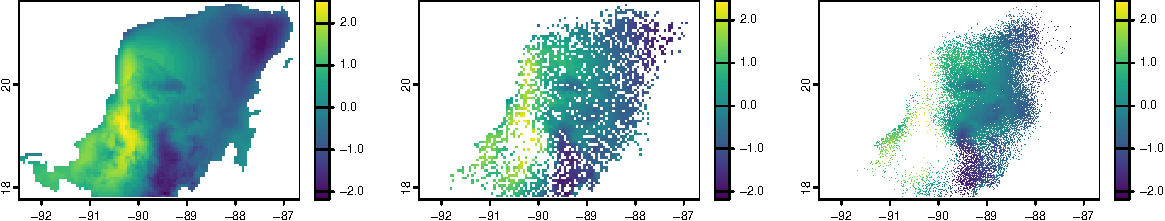
\includegraphics{Tutorial-spatstat-2_files/figure-beamer/unnamed-chunk-25-1} \end{center}
\end{frame}

\begin{frame}{Histogramas}
\protect\hypertarget{histogramas}{}
\begin{center}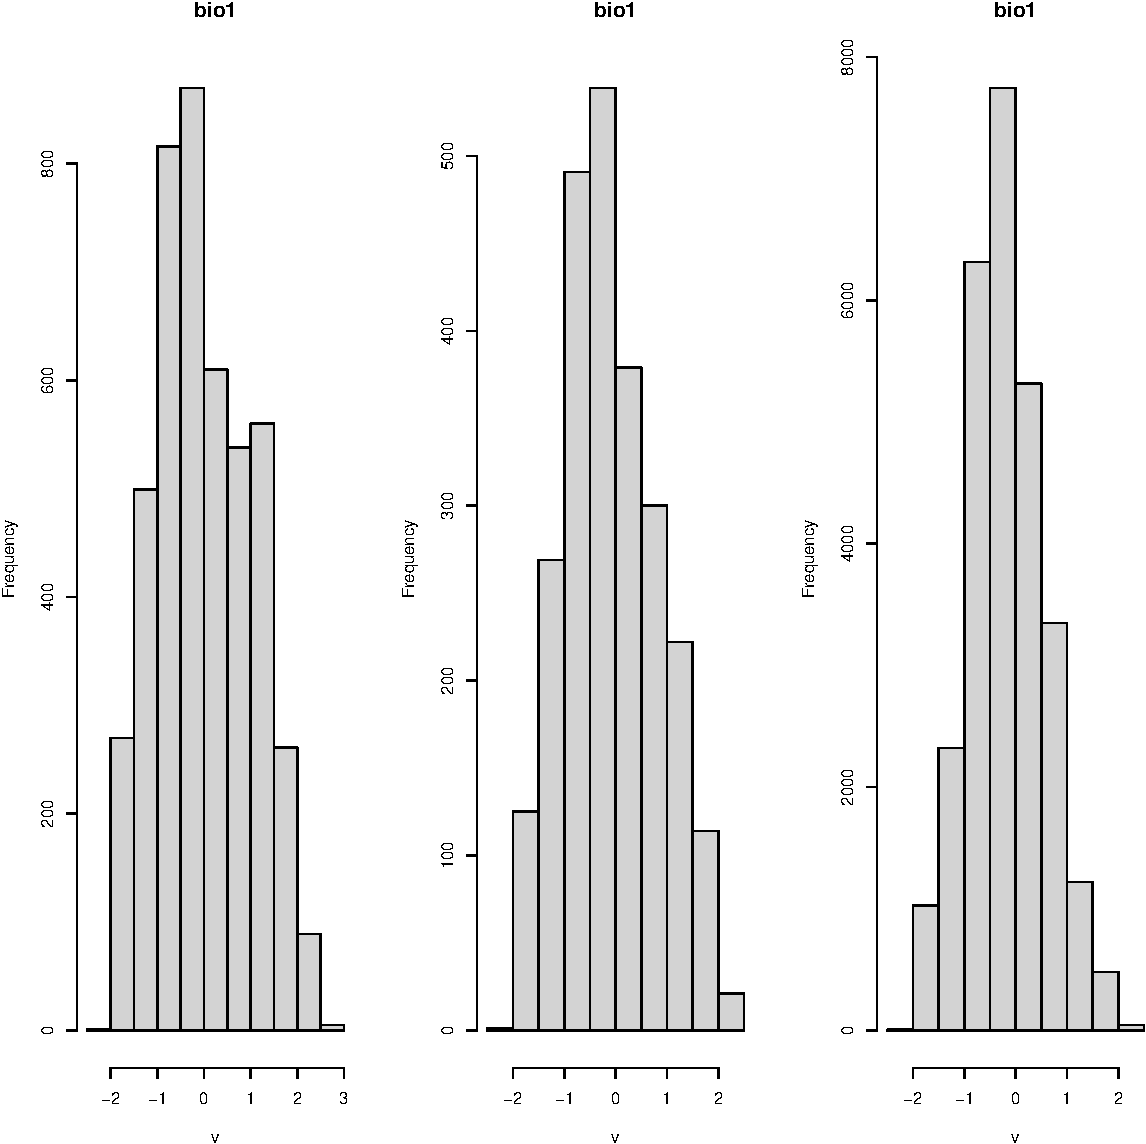
\includegraphics{Tutorial-spatstat-2_files/figure-beamer/unnamed-chunk-26-1} \end{center}
\end{frame}

\begin{frame}{El resto de la historia}
\protect\hypertarget{el-resto-de-la-historia}{}
\begin{enumerate}
\tightlist
\item
  Correr análisis exploratorio con capas filtradas
\item
  Seleccionar exponentes
\item
  Generar fórmulas
\item
  Ajustar modelos
\item
  Evaluar bondad de ajuste
\item
  Proyectar a geografía completa (sin filtrado)
\item
  Validar
\end{enumerate}
\end{frame}

\end{document}
